% This is "sig-alternate.tex" V2.0 May 2012
% This file should be compiled with V2.5 of "sig-alternate.cls" May 2012
%
% This example file demonstrates the use of the 'sig-alternate.cls'
% V2.5 LaTeX2e document class file. It is for those submitting
% articles to ACM Conference Proceedings WHO DO NOT WISH TO
% STRICTLY ADHERE TO THE SIGS (PUBS-BOARD-ENDORSED) STYLE.
% The 'sig-alternate.cls' file will produce a similar-looking,
% albeit, 'tighter' paper resulting in, invariably, fewer pages.
%
% ----------------------------------------------------------------------------------------------------------------
% This .tex file (and associated .cls V2.5) produces:
%       1) The Permission Statement
%       2) The Conference (location) Info information
%       3) The Copyright Line with ACM data
%       4) NO page numbers
%
% as against the acm_proc_article-sp.cls file which
% DOES NOT produce 1) thru' 3) above.
%
% Using 'sig-alternate.cls' you have control, however, from within
% the source .tex file, over both the CopyrightYear
% (defaulted to 200X) and the ACM Copyright Data
% (defaulted to X-XXXXX-XX-X/XX/XX).
% e.g.
% \CopyrightYear{2007} will cause 2007 to appear in the copyright line.
% \crdata{0-12345-67-8/90/12} will cause 0-12345-67-8/90/12 to appear in the copyright line.
%
% ---------------------------------------------------------------------------------------------------------------
% This .tex source is an example which *does* use
% the .bib file (from which the .bbl file % is produced).
% REMEMBER HOWEVER: After having produced the .bbl file,
% and prior to final submission, you *NEED* to 'insert'
% your .bbl file into your source .tex file so as to provide
% ONE 'self-contained' source file.
%
% ================= IF YOU HAVE QUESTIONS =======================
% Questions regarding the SIGS styles, SIGS policies and
% procedures, Conferences etc. should be sent to
% Adrienne Griscti (griscti@acm.org)
%
% Technical questions _only_ to
% Gerald Murray (murray@hq.acm.org)
% ===============================================================
%
% For tracking purposes - this is V2.0 - May 2012

\documentclass{sig-alternate}
% *** CITATION PACKAGES ***
%
\usepackage{cite}
% cite.sty was written by Donald Arseneau
% V1.6 and later of IEEEtran pre-defines the format of the cite.sty package
% \cite{} output to follow that of IEEE. Loading the cite package will
% result in citation numbers being automatically sorted and properly
% "compressed/ranged". e.g., [1], [9], [2], [7], [5], [6] without using
% cite.sty will become [1], [2], [5]--[7], [9] using cite.sty. cite.sty's
% \cite will automatically add leading space, if needed. Use cite.sty's
% noadjust option (cite.sty V3.8 and later) if you want to turn this off.
% cite.sty is already installed on most LaTeX systems. Be sure and use
% version 4.0 (2003-05-27) and later if using hyperref.sty. cite.sty does
% not currently provide for hyperlinked citations.
% The latest version can be obtained at:
% http://www.ctan.org/tex-archive/macros/latex/contrib/cite/
% The documentation is contained in the cite.sty file itself.






% *** GRAPHICS RELATED PACKAGES ***
%
%\if CLASSINFOpdf
  \usepackage{graphicx}
  \usepackage{epstopdf}
 % \usepackage{auto-pst-pdf}
  % declare the path(s) where your graphic files are
  % \graphicspath{{./eps}{./pdf/}{./jpeg/}}
  % and their extensions so you won't have to specify these with
  % every instance of \includegraphics
  \DeclareGraphicsExtensions{.eps,.pdf,.jpeg,.png,.ps}
%\else
  % or other class option (dvipsone, dvipdf, if not using dvips). graphicx
  % will default to the driver specified in the system graphics.cfg if no
  % driver is specified.
 % \usepackage[dvips]{graphicx}
  % declare the path(s) where your graphic files are
  % \graphicspath{{./eps/}}
  % and their extensions so you won't have to specify these with
  % every instance of \includegraphics
 % \DeclareGraphicsExtensions{.eps}
%\fi
% graphicx was written by David Carlisle and Sebastian Rahtz. It is
% required if you want graphics, photos, etc. graphicx.sty is already
% installed on most LaTeX systems. The latest version and documentation can
% be obtained at: 
% http://www.ctan.org/tex-archive/macros/latex/required/graphics/
% Another good source of documentation is "Using Imported Graphics in
% LaTeX2e" by Keith Reckdahl which can be found as epslatex.ps or
% epslatex.pdf at: http://www.ctan.org/tex-archive/info/
%
% latex, and pdflatex in dvi mode, support graphics in encapsulated
% postscript (.eps) format. pdflatex in pdf mode supports graphics
% in .pdf, .jpeg, .png and .mps (metapost) formats. Users should ensure
% that all non-photo figures use a vector format (.eps, .pdf, .mps) and
% not a bitmapped formats (.jpeg, .png). IEEE frowns on bitmapped formats
% which can result in "jaggedy"/blurry rendering of lines and letters as
% well as large increases in file sizes.
%
% You can find documentation about the pdfTeX application at:
% http://www.tug.org/applications/pdftex

% *** ALIGNMENT PACKAGES ***
%
%\usepackage{array}
% Frank Mittelbach's and David Carlisle's array.sty patches and improves
% the standard LaTeX2e array and tabular environments to provide better
% appearance and additional user controls. As the default LaTeX2e table
% generation code is lacking to the point of almost being broken with
% respect to the quality of the end results, all users are strongly
% advised to use an enhanced (at the very least that provided by array.sty)
% set of table tools. array.sty is already installed on most systems. The
% latest version and documentation can be obtained at:
% http://www.ctan.org/tex-archive/macros/latex/required/tools/
\usepackage{balance}
\usepackage{mdframed}
%\usepackage{mdwmath}
%\usepackage{mdwtab}
% Also highly recommended is Mark Wooding's extremely powerful MDW tools,
% especially mdwmath.sty and mdwtab.sty which are used to format equations
% and tables, respectively. The MDWtools set is already installed on most
% LaTeX systems. The lastest version and documentation is available at:
% http://www.ctan.org/tex-archive/macros/latex/contrib/mdwtools

\begin{document}
%
% --- Author Metadata here ---
\conferenceinfo{WOODSTOCK}{'97 El Paso, Texas USA}
%\CopyrightYear{2007} % Allows default copyright year (20XX) to be over-ridden - IF NEED BE.
%\crdata{0-12345-67-8/90/01}  % Allows default copyright data (0-89791-88-6/97/05) to be over-ridden - IF NEED BE.
% --- End of Author Metadata ---

\title{Applying gamification to developer practices}
\subtitle{Why developer habits die hard}
% 
% You need the command \numberofauthors to handle the 'placement
% and alignment' of the authors beneath the title.
%
% For aesthetic reasons, we recommend 'three authors at a time'
% i.e. three 'name/affiliation blocks' be placed beneath the title.
%
% NOTE: You are NOT restricted in how many 'rows' of
% "name/affiliations" may appear. We just ask that you restrict
% the number of 'columns' to three.
%
% Because of the available 'opening page real-estate'
% we ask you to refrain from putting more than six authors
% (two rows with three columns) beneath the article title.
% More than six makes the first-page appear very cluttered indeed.
%
% Use the \alignauthor commands to handle the names
% and affiliations for an 'aesthetic maximum' of six authors.
% Add names, affiliations, addresses for
% the seventh etc. author(s) as the argument for the
% \additionalauthors command.
% These 'additional authors' will be output/set for you
% without further effort on your part as the last section in
% the body of your article BEFORE References or any Appendices.

\numberofauthors{3} %  in this sample file, there are a *total*
% of EIGHT authors. SIX appear on the 'first-page' (for formatting
% reasons) and the remaining two appear in the \additionalauthors section.
%
% author names and affiliations
% use a multiple column layout for up to three different
% affiliations
\author{
\alignauthor
Will Snipes\\
\affaddr{ABB Corporate Research}\\
\affaddr{Industrial Software Systems}\\
\affaddr{Raleigh, NC USA}\\
\email{will.snipes@us.abb.com}
\and
\alignauthor
Anil R. Nair\\
\affaddr{ABB Corporate Research}\\
\affaddr{Industrial Software Systems}\\
\affaddr{Bangalore, India}\\
\email{anil.nair@in.abb.com}
\and
\alignauthor
Emerson Murphy-Hill
\affaddr{North Carolina State University}\\
\affaddr{Department of Computer Science}\\
\affaddr{Raleigh, N.C. USA}\\
\email{emerson@csc.ncsu.edu}\\
}



\maketitle
\begin{abstract}
As software development practices evolve, we face the continuous challenge of communicating new practices and tools to the community.  As developers, we both like to try new things and like to stick with the familiar.  In addition to training, discussing, and presenting software engineering practices and tools, we seek to communicate them through active two-way information embedded in the Integrated Development Environment (IDE).  While communicating, we also collect data on new and current practices and tools used by each developer by recording actions in the IDE.  With a rich data source, we evaluate what practices are used, define metrics that give individual feedback, and create an environment where developers can see how they are doing compared with their teammates.  

This approach helps understand practice and tool use over the long term and judges the lasting change a communication effort makes in everyday habits.  Tool support provides a mechanism to embed into Visual Studio an extension that provides the capture of usage data while giving feedback to users on their practices both in general and specific to the ones being promoted.  Through a points score system that assigns points to specific commands and tools we encourage everyone to use the new practices.  Providing a light score ranking view should help us stay motivated as we compare our command usage to our peers.  To demonstrate how this works, we implement a longitudinal study that demonstrates the results from this approach as we engage with developers over a month-long period.  

Results from this demonstrative study show that in general the approach is <blank> with a few developers <blank> of the study.  The effectiveness of this approach for communicating about practices is demonstrated through the continued use of the commands as we communicate them.  Evaluation of metrics for navigation ratio over time show that developer use the commands <blank> than they did during the benchmarking phase.  The result of the study shows that this method for communicating and promoting software engineering tools and practices <blank>.
\end{abstract}

% A category with the (minimum) three required fields
\category{H.4}{Information Systems Applications}{Miscellaneous}
%A category including the fourth, optional field follows...
\category{D.2.8}{Software Engineering}{Metrics}[complexity measures, performance measures]

\terms{gamification}

\keywords{empirical, training, learning, usability}

\section{Introduction}
%update
Deploying these techniques requires communicating and motivating developers to use them.  Murphy-Hill and colleagues  \cite{wbsnipes:Hill2011Peer} show that developers can effectively learn about new tools from their peers by watching them work and through recommendations, yet this happens very rarely, in part because developers rarely work on the same computer at the same time.  This personal connection limits the knowledge transfer to the co-located circle of colleagues connected with the early adopters.  



\section{Assess the Viability of Gamification for Software Engineering}

\subsection{Assessment Background}
When discussing gamification, folks raise a concern about replacing an activity that is intrinsically motivated with extrinsic motivation provided by points and achievements.  To discover what is behind this concern, several studies are useful to understand what should be done. 

Early studies attempt to evaluate achievement motivation in students and relate that to their performance in school.  The study by Hermans describes results from applying questionnaire to evaluate achievement motivation in students \cite{wbsnipes:Hermans1970Questionnaire}.  Each question is ranked for its correlation to achievement motivation. Results indicate that some key questions about the diligence with which students approach their work are correlated with achievement motivation.  The questions in this questionnaire and their ranking may be useful for evaluating achievement motivation in further studies.  Take care when choosing appropriate questions that for the context of the survey.

Maehr proposes an affirmative theory that individuals achieve as a member of a social group choosing the behavior that will meet the expectations and values of the group that is significant to them. \cite{wbsnipes:MaehrCulture}  So the presence of a social group where the person is motivated to belong and excel within is important for creating achievement motivation.  Maehr states that since achievement behaviors can be triggered by circumstance, that they are present in most people regardless of background. 

Beecham and colleagues provide a thorough analysis of existing literature on studies of motivation in Software Engineering\cite{wbsnipes:Beecham2008Motivation}. It has some valuable lists of factors that motivate software engineers with the most common being "the work" motivates us. The list of de-motivators is also useful with common job satisfaction items like stress and inequity in recognition, plus poor quality software (low accomplishment) and lack of influence in decision making. The paper also lists characteristics of people in the professions including need for independence (autonomy), desire to learn new skills/tackle challenges. 

Understanding the concerns with maintaining intrinsic motivation while adding elements of achievement motivation, we developed an assessment survey questionnaire to determine whether the community would be receptive to a gamification approach to software development.   We designed  the survey to assess how developers are motivated to use training, practices, and tools and whether they are open to having that information shared with their peers and managers, and being recognized with badges and points. The developer study conducted with over 130 software developers at ABB challenged whether achievement motivation would help software engineers and whether they would accept sharing data on tools and practices they use to help others.

\subsection{Assessment Results}

Using a question from the Saachi and Saachi survey\cite{wbsnipes:SaatchiGameification} as directly as possible, we asked developers at ABB "How interested they would be in working for a company that incorporated some aspects of games into software engineering tools as a way to increase productivity in the workplace"?  We segmented results by country in Figure \ref{fig:gamification} and found that gamification of software engineering is more interesting to developers in India, Poland, and Finland than in other major countries.  The responses indicating that developers were at least somewhat interested is 75-88\% In India, Poland, and Finland.  For the US, Sweden, and Switzerland the responses indicate 60-65\% are at least somewhat interested.  The overall ABB response is comparable to the Saachi and Saaschi survey\cite{wbsnipes:SaatchiGameification} upon which this question was based that found 75\% of 18-45 year olds were at least somewhat interested.  

\begin{figure}\begin{mdframed}[linecolor=white]
	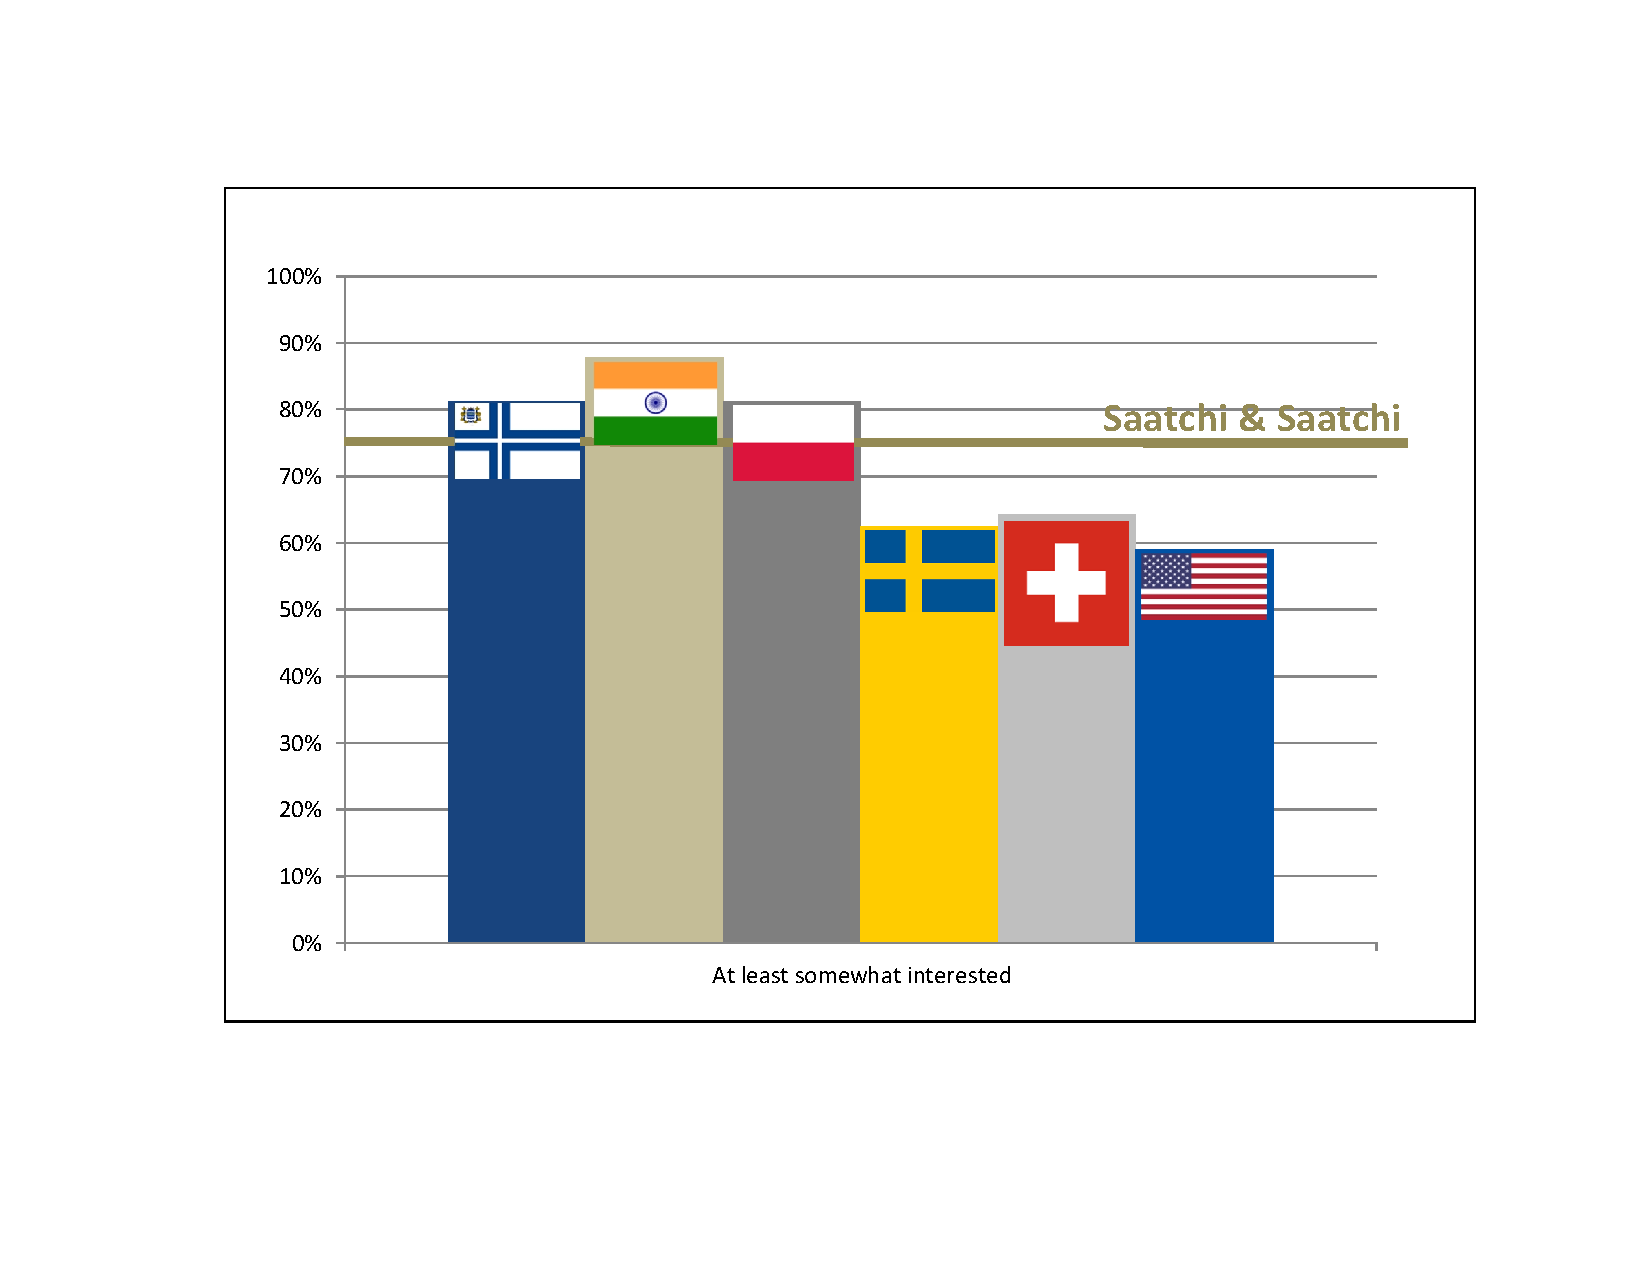
\includegraphics[width=3in]{gamificationquestion.pdf}
	\caption{Acceptance of gamification}
	\label{fig:gamification}
\end{mdframed}\end{figure}

We asked developers how likely they would be to try tools and practices recommended to them through an automated usage tracking system.  Answers showed that 95\% of the developers surveyed are likely to try tools and practices recommended to them.  This indicates that a recommendation system would positively impact the deployment of software engineering tools and practices at ABB.

One area we questioned was whether sharing detailed usage information with colleagues and the company as a whole would be a concern for developers.  A graduated scale was used for the community that would be shared with and distinction between whether that sharing was anonymous or the information was personally identifiable. Figure \ref{fig:comfortwithsharing}  shows that over 90\% of respondents are comfortable with sharing either anonymous or non-anonymous information with their team members. 
Their comfort level decreases as the scope of who the information is shared with increases.  People were less comfortable sharing with anyone (the category for people outside ABB) particularly if the data were not anonymous.  
Two conclusions from this feedback are that people are very willing to share information that could help their team. Second, sharing within the company is acceptable if we take care to make the data anonymous.

\begin{figure}\begin{mdframed}[linecolor=white]
	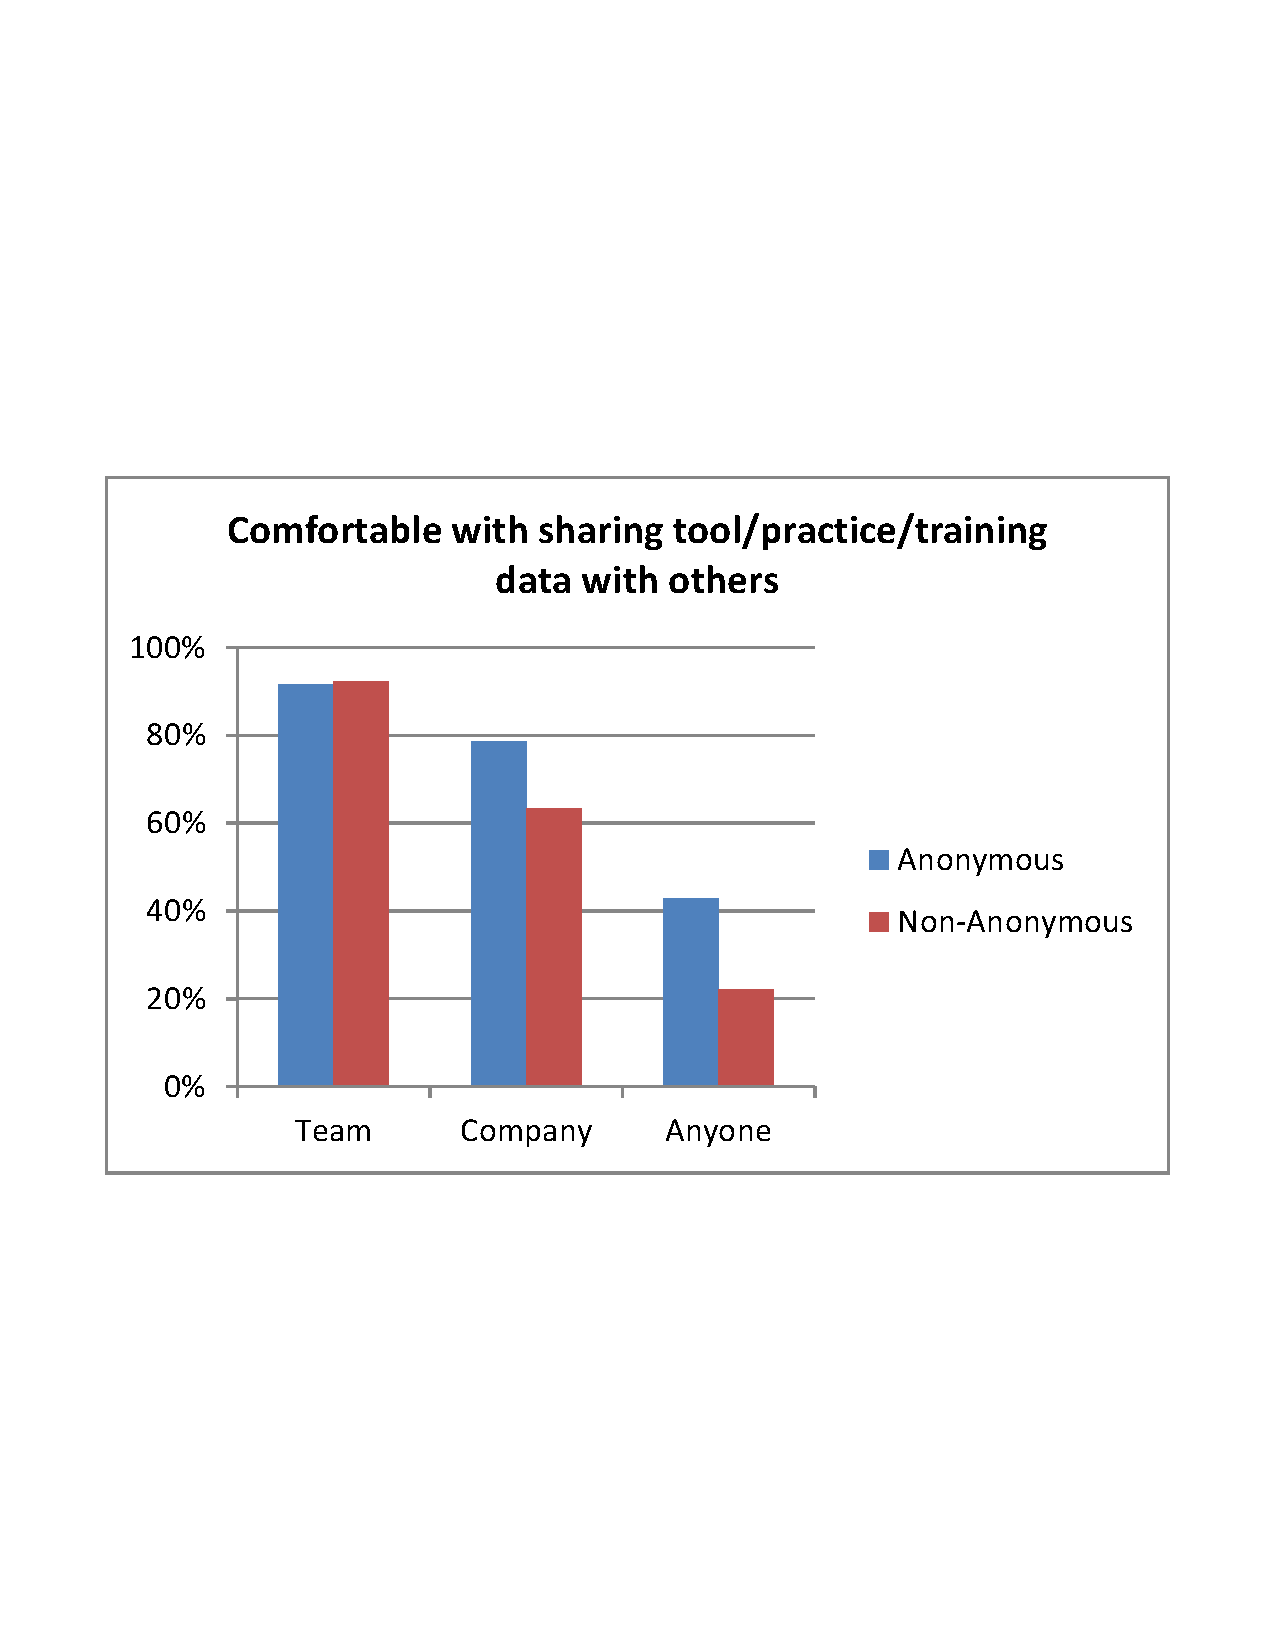
\includegraphics[width=3in]{ComfortWithSharing.pdf}
	\caption{Comfortable with sharing usage information}
	\label{fig:comfortwithsharing}
\end{mdframed}\end{figure}

Developers were asked what would motivate them to use tools and practices and given 4 choices to rank.  The top motivator for using tools and practices is coworker recommendation with 75\% of respondents in Figure \ref{fig:toolandpracticemotivators}   ranking in 1st or 2nd place. The lowest was having badges posted on their social profile where 33\% ranked this in 1st or 2nd place.   Badges also ranked low in motivations for taking more software engineering training.  We conclude that a facility to share coworker recommendations on tools and practices has the best opportunity to increase their adoption.  Since a competition among teams ranks slightly higher than management mandate, we have the choice to apply one or the other or both as motivation for using key practices.  
 
\begin{figure}\begin{mdframed}[linecolor=white]
	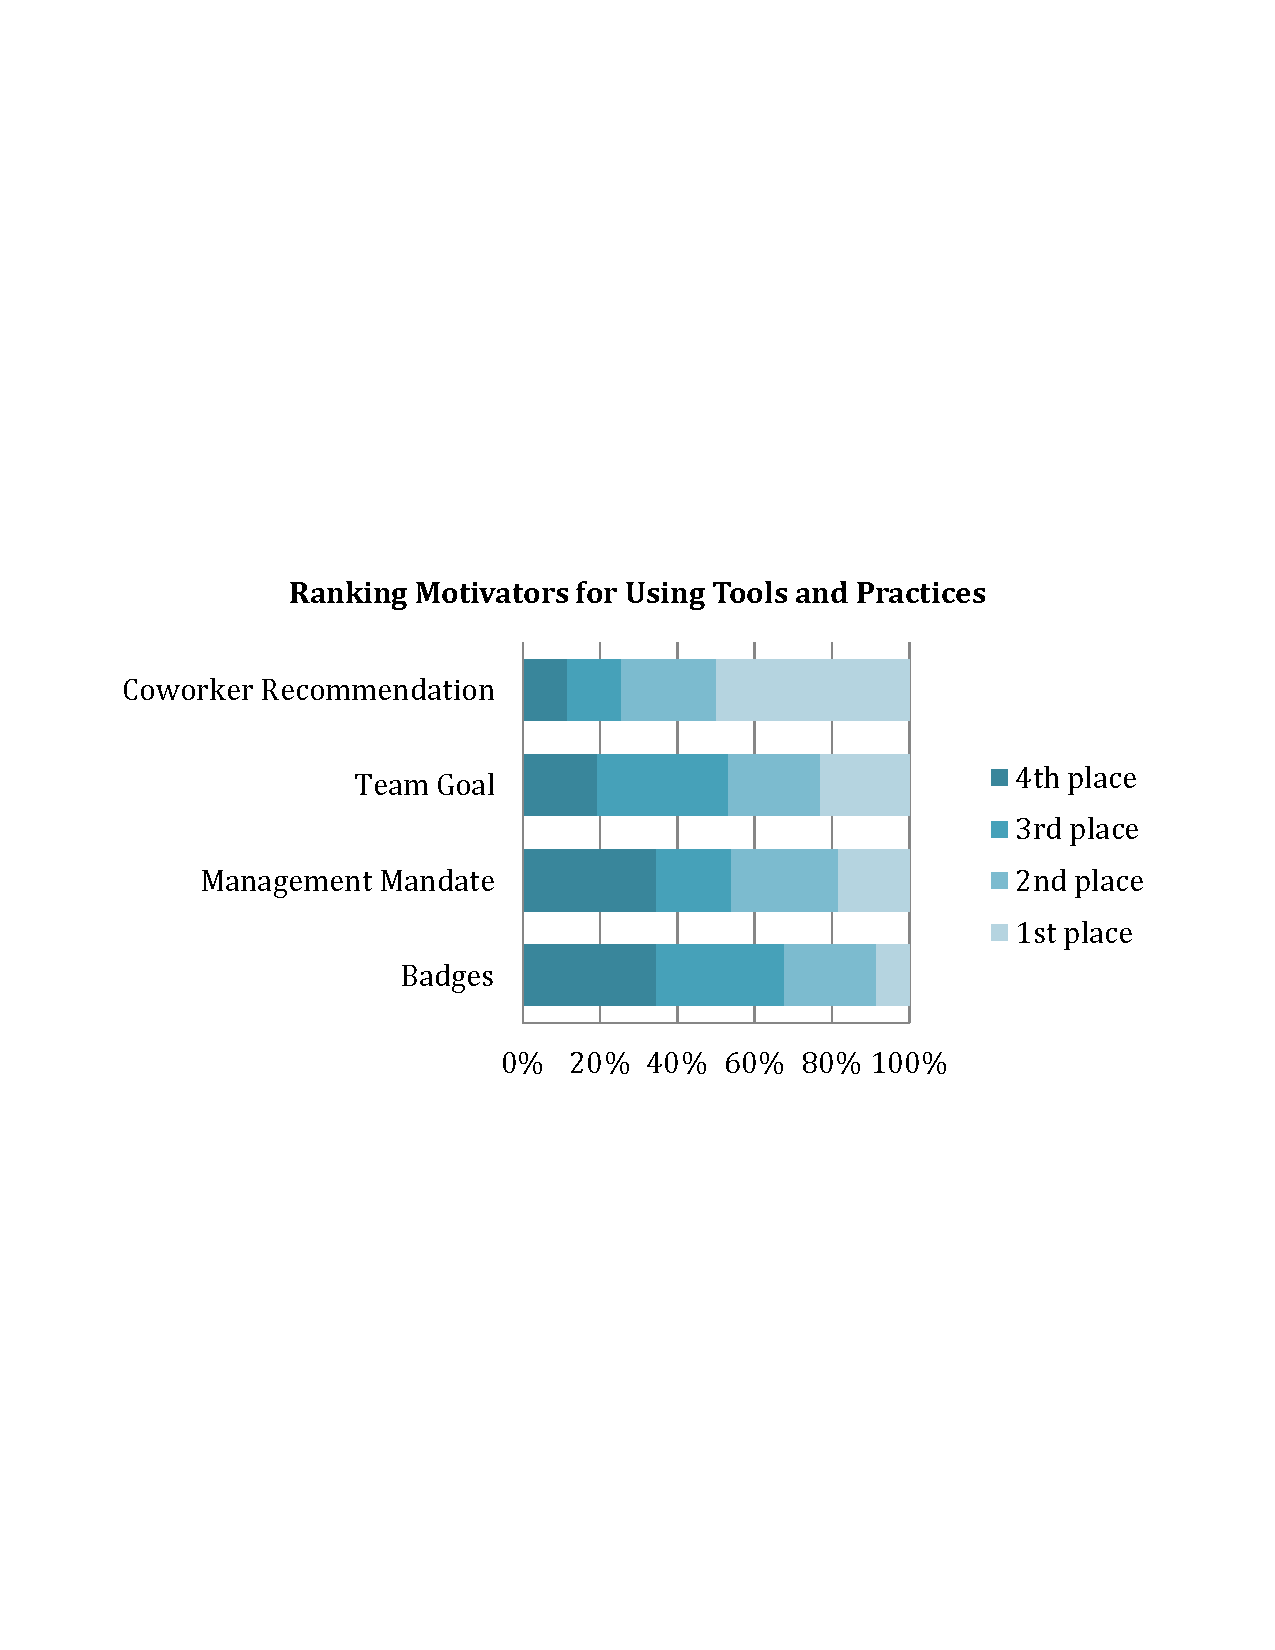
\includegraphics[width=3in]{ToolAndPracticeMotivators.pdf}
	\caption{Motivation for using tools and practices}
	\label{fig:toolandpracticemotivators}
\end{mdframed}\end{figure}

Developers were asked to rank awards for different actions by which they would find the most desirable.  Overall 68\% of developers ranked receiving an award for consistently performing quality practices as either 1st or 2nd place.  This supports a conclusion that focusing on awarding quality practices would motivate developers to do them consistently.
 
Based on the survey results we made the following conclusions:
•	95\% of developer responding would try tools and practices suggested by an automated recommendation system particularly if they were provided in context with the current workflow pattern the developer follows.
•	Responses indicate a preference for team competition over individual awards (badges) and awards for quality practices ranked highest.  So, the tool will incorporate team competition ideas and recognize quality practices.
•	Over 90\% of respondents approved of sharing data with their team members


\section{Study and Game Design}

Utilizing the unobtrusive continuous monitoring capabilities of Blaze, we designed the pilot as a longtiudinal study in three waves.  Longtiudinal studies allow us to design an experiment and determine the effects over two or more sample periods using standard MANOVA (Multiple ANalysis of VAriance) models. \cite{longitudinalbook}  We employed the three wave model defining the first wave as a baseline capturing the current practices of the pilot group.  The second wave employed the intervention that included an informative web site on structured navigation commands in Visual Studio, information about the Sando search tool, and information about how points would be awarded during the pilot.  The third wave provided the participants with continuous feedback in the from of points accumulated and an indicator arrow \ref{fig:blazegui} that points up when their navigation ratio is higher than their historical average.  

Developing the study with the available tooling means that we follow steps as follows.
1. Define the practice we wish to measure compliance with
2. Develop a mapping of the practice to actions that are captured by the blaze tool from the IDE
3. Weight the actions according to their importance to the practice and assign points to the actions in the configuration file
4. Develop the intervention method
5. Determine the phases and length of the phase in the study according to baseline, intervention, and continuous feedback
6. Select participants to deploy
7. Define a pre-study questionnaire if one is necessary to collect associated information
8. Define a post-study questionnaire if necessary to collect post study information
9. Communicate with the participants about the study
10. Execute the study and report results

\subsection{Select a Practice}
In their paper on game design patterns, Hamari et. al. issue a warning that assigning achievements to required tasks reduces intrinsic motivation because player autonomy is reduced by the achievements \cite{wbsnipes:Hamari2011Framework} .  This warning indicates that we should avoid giving points for things that are already an expected deliverable such as finding or fixing bugs, completing development tasks, or meeting required process criteria.  Practices to consider are those practices with room to go beyond a checklist or minimum criteria where developers have the opportunity to excel.

Selecting a practice to study involves identifying a practice, defining specific characteristics of the practice to measure, and identifying the actions in Visual Studio that relate to the practice.  We currently limit ourselves to practices that exist entirely in the IDE thus can be monitored using Blaze.  We identified potential practices of test-driven development, debugging practices, navigation practices,  eliminating static analysis bugs, and check-in frequency.  Practices of check-in frequency, static analysis bug elimination are highlighted in this paper's related work section with prior gamification studies in classroom environments.  Johnson and Kou achieved automated monitoring of test-driven development practices with Zorro thus may provide a candidate for future gamification application.   Debugging practices have developer community opinions on optimal methods, however, detailed debug practices with modern IDEs have not received research community attention, thus are also reserved for future work.  Based on studies of structured navigation by Robillard et. al. that identify structured navigation as a practice leading to effective program maintenance  \cite{wbsnipes:Robillard2004How}, we identified structured navigation as a key practice.   Structured navigation fits the requirement of a practice that is contained in the IDE, is something that has proven benefits, and lends itself to measurement and scoring, is not an assigned task, and leaves room for developers to excel.  

\subsection{Design the Game}

To setup the game for a practice, the Blaze tool provides an XML configuration file where the researcher can configure Blaze to categorize and assign points to the commands that are part of a software engineering practice.  Blaze allows the researcher to define multiple command category levels.  Thus we can categorize commands that are navigation then further classify them into structured and unstructured navigation.  We categorize commands as structured navigation when they allow the developer to locate a code element following the program structure from another element.  For example, Navigate To \textit{Ctrl+,}, Go To Definition \textit{F12}, and Find All References \textit{Ctrl+K,R} are commands that follow structure of the code, which we classify as structured navigation.
Commands that we considered as unstructured navigation include scrolling through a file using keys or the scroll-bar, opening files from the Solution Explorer, Find commands (e.g. Find in Files), Go-to line number, and children of these commands (e.g. Find Next).

Gamification practices consider the feedback of achievements and points as critical to a successful outcome.  The design of achievement awards should gradually encourage the participant to reach higher and higher levels of success in the activity.  Achievements must feel earned to the participant so that internally they recognize the effort to get the award was significant and feel satisfied  \cite{wbsnipes:Hamari2011Framework}.  Hamari and Eranti describe a general relationship between achievements in games and regular game play      In games achievements are typically a parallel scoring system to the main game play.  They make the game more engaging providing multiple ways to increase your score and multiple challenges in one interface.

Using these guidelines we assigned points to structured navigation commands which received 1-10 points each while unstructured navigation commands received 0 points.  Assigning negative points is discouraged as this may demotivate folks who do not have detailed knowledge of how the points are assigned.\cite{}   In creating levels, following the guidance from Hamari \cite{wbsnipes:Hamari2011Framework}, we built levels following an exponential curve.  Users initially level up after a working day or two extending to achieving the next level after a week or even a month following an exponential curve.  The levels make the game motivating for beginners and challenging for more experienced developers.  We designed the points and levels such that above average developers can complete all levels during the study period.

\subsection{Intervention Staging}

After selecting the practice to focus on, we needed to select an intervention method.  The term intervention, indicates that we are applying a technique to influence a change in the measured behavior of developers.  Intervention involves communication about the practice in a way that motivates adoption \cite{}.  Interventions can include presentations, one-on-one discussions, distance education mechanisms such as webinars, and word of mouth recommendations.  Part of the research objective is to determine whether we can achieve adoption of a practice with alternative interventions that are more deliberate than word of mouth and perhaps more scalable than webinars or presentations.  

In the initial wave, participants were informed of the purpose of the study what to expect from the Blaze tool.  The participants installed the tool in their Visual Studio environment.  The tool did not present any window for them to see and simply collected data in the background.   

After a week's data collection marking the end of the first wave, Blaze started to automatically pop-up a window containing a button for a web page with information.  The page included a link to download another tool for code search called Sando \ref{sando} and information about using that tool in a video.  The sub-page on navigation contained a page of tutorial on the built-in structured navigation commands in Visual Studio.  The About Blaze page contained details of the point scoring system and background on Blaze's purpose.  The usefulness of the communication site is rated as part of our study completion survey.

In the third wave developers received instant feedback from Blaze on the points they accumulated during the development session.  The up/down arrow provided a simple indicator on whether they were increasing their use of structured navigation or were using it less than their personal historical average.  This final configuration continued until the end of the pilot.  

\subsection{Participants}

We conducted this study with an intact team of developers working in an R\&D facility in India on a large industrial software system.  Developers were asked to volunteer for the pilot by their management, however, managers did not know who participated in the study.  Mechanisms in our data collection to identify individuals were under the control of each developer, they could chose to share or keep confidential the association of a generated unique id with researchers or each other.  

Management wished to have no knowledge of who was participating and took great care to remain detached from the pilot proceedings.  Data at this level of detail has not been collected in ABB development organizations except for a few minutes of video study that might be conducted.  Researchers were careful to create the system so that developers controlled their identification with the data and fortunately, management bought into the necessary anonymity of the participants.

\subsection{Competitive Elements}
By selecting an intact team, we hope to leverage aspects of motivation such as the Leaderboard to spur feelings of competition among teammates.    The leaderboard was presented so that developers could see their own score in relation to the top 5 people on the leaderboard.  However, the identifier of the other participants was generated as 3 capital letters assigned based on their position on the leaderboard.  Therefore the assigned letters could even change when an individual's ranking changed.  Not knowing who of your colleagues was ahead of you could be a factor in motivation, but also avoids one potential source of conflict in an intact team.

Competitive dynamics may be more effective when teams from different areas can compete as a team against other teams..  This tried and true method both builds esprit de corps and enhances achievement towards the intended outcome.  This study design is potential future work. 

\section{Related Work}
%update and expand

Johnson and Kou defined Zorro\cite{V:Johnson2007Automated}, a system for detecting whether developers use Test Driven Development techniques based on data from Hackystat.  Zorro divides development activities into episodes delimited by events such as configuration management code check-in, start of a unit test run, or start of a build.  Using the distinct events that developers follow within these episodes, Zorro determines whether the episode followed Test-Driven Development practices per their classic definition of test first - code - test pass, or a different scenario.  In two student-based studies comparing Zorro classifications with a simultaneous observational screen video, Zorro achieved between 70\% \cite{Kou2010Operational} and 89\% \cite{V:Johnson2007Automated} accuracy in classifying episodes into their proper TDD scenarios.  The studies did not, however, attempt to use or evaluate the influence of instant feedback aimed at encouraging participants to follow the classic definition of Test Driven Development.  In our study, we attempt this leap to present data collected directly to developers attempting to influence them to change their practices.

Murphy-Hill, Parnin, and Black \cite{V:MurphyHill2012How} use the Mylyn Monitor to explore whether or not developers use the automated refactoring tools present in Eclipse.  They look for specific refactoring commands in Eclipse and determine the amount of time developers use tools versus hand refactoring the code.  For this study we build a tool that captures the use of all commands within the Visual Studio environment including refactoring, navigation, and edit commands.

Robillard, Coelho and Murphy explore hypotheses around how developers can be more effective at performing a maintenance task \cite{wbsnipes:Robillard2004How}.  Key conclusions are that developers are more more successful finding and fixing bugs when they create a detailed plan for implementing a change, use structured navigation with keyword search or cross-reference search, and only review methods once during their search.  This builds on this work by testing methods for increasing the use of structured navigation in developers everyday practice.

Singer and Schneider demonstrate the use of a message board and points for encouraging students to increase their frequency of commits to the source code repository.\cite{Singer2012It}  The communication mechanism enabled students to see each others' progress and resulted in more frequent commits than baseline.  Participants valued the communication and collaboration aspect and some valued the competition enough to change their opinion on optimum commit frequency.  The subsequent thesis by Singer \cite{Singer2013a} describes results of an experiment conducted across two iterations of a class where active feedback on commits was deployed to one course and another course served as the control group where commit frequency was simply monitored.  Results show an increase in the frequency of commits at a statistically significant level.  This study uses fine grained instrumentation to identify practices used between commits such as structured navigation.

The Pro Metrics (PROM) tool provides a framework for collecting data for further analysis from tools used by developers.\cite{Coman2009Casestudy}  It provides a flexible data model and a plug-in architecture to facilitate collection from different data sources.  Studies conducted using prom include a series of studies by it's creators on trends in time spent Pair Programming \cite{Coman2008Investigating}, benefits of refactoring on productivity \cite{Moser2008Case}, impact of refactoring on re-usability \cite{Moser2006Does}, and prediction of effort \cite{Abrahamsson2007Effort}.  The PROM tool and studies that use it track the time spent editing files and methods from the IDE and code metrics obtained trough source code analysis.  Applying these data to specific research questions such as whether refactoring improves productivity \cite{Moser2008Case} shows the utility of combining automated effort data with code metric data.  Taking a different focus on techniques, our study used more detailed events captured from the IDE  to detect how the user was navigating through the code in addition to knowing how long the editor is open for a particular file.

Murphy-Hill et. al. study a large usage history data set and apply several different algorithms to accurately suggest to users new commands in their environment to use.\cite{MurphyHill2012Improving} Algorithms based on command history performed well particularly when synchronized chronologically with the recipient's usage history. Novice users were better served by recommendation algorithms that did not require a long history, where more expert users benefited from more sophisticated algorithms that included more history. The "Most Widely Used" algorithm that recommends commands based on the collective usage profile of the team performed nearly as well as the more sophisticated algorithms. The paper presents the methodology for making recommendations and the evaluation of the accuracy of the recommendations. Our work goes the next step of evaluating whether a specific recommended practice gets adopted by developers when influenced through gamification methods.

Dubois and Tamburrelli discuss theoretical concepts behind applying gamification to software development. \cite{Dubois2013Understanding} Their approach is to consider how gamification could be applied throughout the software development life-cycle to motivate many practices in different phases.  They provide guidance on assessing gamification in the software development domain that includes analyzing the actors and game mechanics, defining integration with existing tools and processes, and designing the evaluation of results.  Dbois and Tamburrelli demonstrate this guidance using a study of students working on a class project.  Defining a control group and subject group of students, both groups receive the same feedback about their code comments, test coverage, code size, and static analysis rule violations.  The subject group can see each others' rankings while the control group only sees their personal rankings.  Results though inconclusive indicate that competition increases the desired results.  In our study we apply both individual feedback and competitive based feedback (anonymized) to participants and seek to observe a change in their behavior after an intervention.

\section{Results}

Although we translated navigation commands to points for developers, we defined the metric Navigation ratio based on Jones and Jones \cite[] as the number of structured navigation events in a day over the number of unstructured navigation events.  This metric provides a continuous variable allowing us to use statistical data of continuous data to check our hypotheses.  To create the evaluation for each wave, we took the navigation ratio for each developer in each wave.

The following hypotheses interest us in the current study.  
1. Developers using blaze use more structured navigation when they receive instant feedback about their practices
2. Developers find the competitive aspect of blaze encourages them to pay more attention to navigation practices

To evaluate whether developers use more structured navigation when they receive instant feedback, we monitor the change in navigation ratio over the pilot study period.   Expecting that as developers learn about navigation commands and tools that count towards the score in the second week they will begin using the practices more.  Also expecting that noticing the leaderboard competition will encourage some developers to use the navigation practices more.  What we observed is shown in Figure \ref{fig:navigationaverage} that the structured navigation practice did not increase significantly from the beginning to the end of the study.  Overall, we did not see a significant effect towards increasing navigation ratio for the interventions in wave 2 or wave 3.   

\begin{figure}\begin{mdframed}[linecolor=white]
	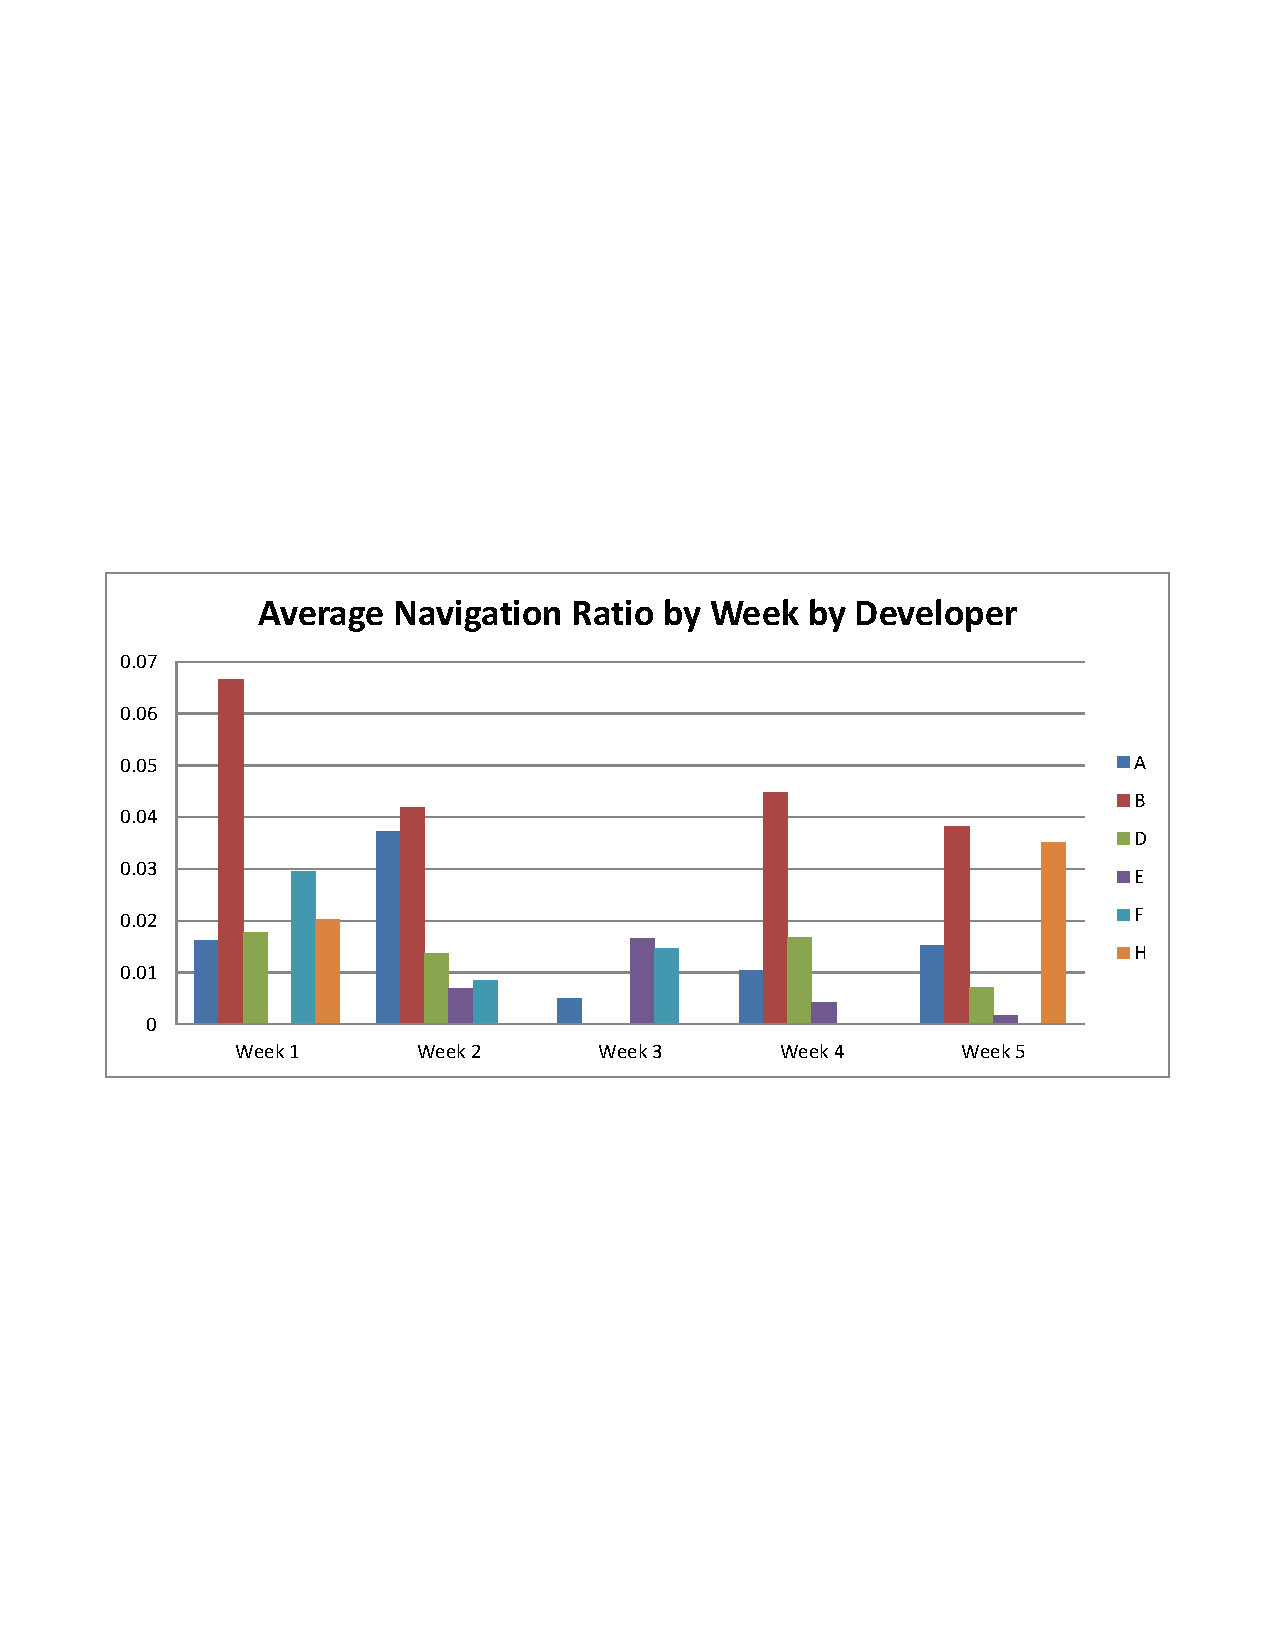
\includegraphics[width=3in]{navigationaverage.pdf}
	\caption{Average Navigation Ratio by Week by Developer}
	\label{fig:navigationaverage}
\end{mdframed}\end{figure}

Is this a spectacular fail from a gamification effectiveness perspective?   How could this be when pre-study results indicated very positive attitudes towards the approach?  Our post pilot survey attempts to shed some light on the reasons.  One question in the post survey is how knowledgeable the developer was about the code they worked in with 3 possibilities,  they were authors of the code, they regularly maintained the code, they were unfamiliar with the code.  In this team, x\% of developers cited that they ...the code.  Another factor to consider is experience level which we also asked in the post-pilot survey.  More experienced developers may be more convinced of their effective habits and perhaps react almost with muscle memory to use structured or unstructured navigation to locate code of interest.  Even developers whose navigation ratio  was lower than average, used structured navigation occasionally as much as their more frequently using colleagues.  The variation for each individual can be seen in Figure \ref{} .

\section{Threats to Validity}
There are several threats to validity for this result.  By making the purpose of our measurement and contest known although without details we may have triggered the participants to think about navigation commands they use before establishing a baseline.  We attempt to control for this by comparing the pilot participants' data to data from Blaze users who are knowledgeable Visual Studio developers but did not receive the interventions.  Another threat is the intact team represents people with different backgrounds and experience levels who may have established habits for navigating through source code.  We attempt to control for this by asking post survey questions of the participants about their familiarity with the code they work in and their experience levels.  The threat of non- generalizable of results remains particularly because the pilot was conducted within an intact team in a single industrial site in India. As the pre-study questionnaire shows, the developer's desirability for a gamification type of intervention vary by country.

\section{Conclusions}
This paragraph will end the body of this sample document.
Remember that you might still have Acknowledgments or
Appendices; brief samples of these
follow.  There is still the Bibliography to deal with; and
we will make a disclaimer about that here: with the exception
of the reference to the \LaTeX\ book, the citations in
this paper are to articles which have nothing to
do with the present subject and are used as
examples only.
%\end{document}  % This is where a 'short' article might terminate

%ACKNOWLEDGMENTS are optional
\section{Acknowledgments}
This section is optional; it is a location for you
to acknowledge grants, funding, editing assistance and
what have you.  In the present case, for example, the
authors would like to thank Gerald Murray of ACM for
his help in codifying this \textit{Author's Guide}
and the \textbf{.cls} and \textbf{.tex} files that it describes.

%
% The following two commands are all you need in the
% initial runs of your .tex file to
% produce the bibliography for the citations in your paper.
\bibliographystyle{abbrv}
\balance
\bibliography{paper_id1} 
 % sigproc.bib is the name of the Bibliography in this case
% You must have a proper ".bib" file
%  and remember to run:
% latex bibtex latex latex
% to resolve all references
%
% ACM needs 'a single self-contained file'!
%

\end{document}
